\chapter{Background}
\label{chp:background}

In this chapter we'll discuss some technical aspects of video conferencing that affects how we reason about the problem, and evaluate what sort of trade-offs established actors on the market have made.

\section{WebRTC}

This thesis is largely inspired by the efforts of the \gls{w3c} on \gls{webrtc}, a technology which enables direct browser-to-browser communication. Building on \gls{webrtc}, services like Telenor Digital's appear.in and Telefónica's Hello have come to life, ushering in a new age of communication that does not depend on the traditional GSM infrastructure, but is fueled by faster Internet connections and more capable smartphones. WebRTC is not a finished standard yet, which is why browser support is variable at the moment, but it's expected that support will become more widespread once the specification is finished\footnote{The current status is ``working draft'', the full specification can be found here: \url{http://www.w3.org/TR/webrtc/}}.

It's interesting to note that many of the largest WebRTC communication platforms (like appear.in and Hello, as mentioned) we've seen so far have been developed by the largest players in the traditional communication field, and not from any independent outsider. The big telephone companies do have capabilities other actors don't enjoy, such as being able to freely route calls back over GSM as a fallback solution in case a person is not reachable online, but this has not been a big selling point for the services so far. The services have also largely been focused on video conversations, even though the technology is equally well-suited for pure voice conversations or text-based communication.

In any case, the hard part of the problem is video conversations, as the demands on the user equipment and the connection is far greater than what will ever be exercised by voice or text. Many services are today artificially limited in size, but often the parties in a conversation will experience trouble before reaching those limits, as their devices have insufficient bandwidth or their CPUs are not capable of encoding enough video streams in parallel.

There are three different implementations of the WebRTC specification that are in extensive use; \texttt{libjingle}, which powers Chrome and Opera; Mozilla's, which is tightly coupled with Firefox; and OpenWebRTC, a mobile-first framework for native apps, started by Ericsson Research. There's also WebRTC Microstack\footnote{\url{http://opentools.homeip.net/webrtc}}, but they only provide the data-channel, which means they don't support the audio/video APIs. Some interest for a pure JavaScript implementation has been expressed to ease development of WebRTC-aware server-side applications\footnote{\url{https://github.com/webrtcftw/goals/issues/1}}, but that project has not seen much activity since late 2014.

Codec issues have been a heated debate for online video, which we will not reproduce in full here. In summary there's two contenders, H.264 and WebM. The WebM project produces the VPx codecs, which are royalty-free and thus preferred by most browser vendors. H.264 is patent-encumbered and requires licenses for use, but is widely deployed due to its usage on BluRay-discs, most TV-content, etc. Both have their pros and cons, but the web community seems to be slowly moving towards WebM\footnote{The Chromium project announced in 2011 that they would remove H.264 support from the browser, but this has not yet happened. \url{http://blog.chromium.org/2011/01/html-video-codec-support-in-chrome.html}}.


\section{A Technical Look at Video Conversations}

\subsection{Encoding}

The naïve approach to encoding video is to encode the raw stream from the web camera into several client-optimized streams for transmission. However, H.264 can be encoded with \gls{svc}, which layers several streams with different bitrates into a single stream. A node receiving a \gls{svc} stream can then extract layers with the bitrate desired, without re-encoding the entire stream. With VP8 this is sadly not possible, and the only alternative is to send several streams with varying bitrates in parallel. This is not as efficient as sending only a single stream, and the encoding step is costlier in terms of CPU-time. This makes nodes like \glspl{sfu} more expensive to run with VP8, as splitting a video stream requires decoding and re-encoding the data.

Google has entered a collaboration with Vidyo \cite{vp9-vidyo} to bring \gls{svc} to VP9, which might bring free-to-use \gls{svc} to WebRTC. While both Firefox and Google support decoding VP9 today \cite{vp9-support}, encoding is not yet supported for either.

Both H.26x and VPx can be hardware-accelerated, and are deployed in several products on the market. Most deployed solutions are decode only, but some, like the Nvidia Tegra 4, also supports encoding \cite{nvidia-hw-encode}. The WebM project maintains open designs for hardware encoders and decoders for VPx.


\subsection{Continuous Presence vs. Voice-Activated Switching}

There are mainly two different ways to do video conversations, Continuous Presence and \acrfull{vas}. Continuous Presence means that all parties in the conversation are visible to all other parties at the same time. \gls{vas} means that only one party is visible, typically the one detected by the system as talking at any given time. There's also hybrid schemes, like Google Hangouts, where all parties are shown to everyone, but the active speaker is shown bigger than the rest. Each node can override locally who's shown up big.

Clearly, in larger conversations, there's a huge difference in network impact of the two technologies, as a VAS-based solution will always just require a single video link in and out, while Continuous Presence requires bandwidth to scale linearly with the size of the conversation. \autoref{fig:service-possibilities} summarizes the possible services that can be provided for different amounts of available bandwidth. A minimal video unit is the smallest bitrate it makes sense to encode video in. This will be service dependent, but we can imagine $\approx$400 kbps to be reasonable.

\begin{figure}
    \centering
    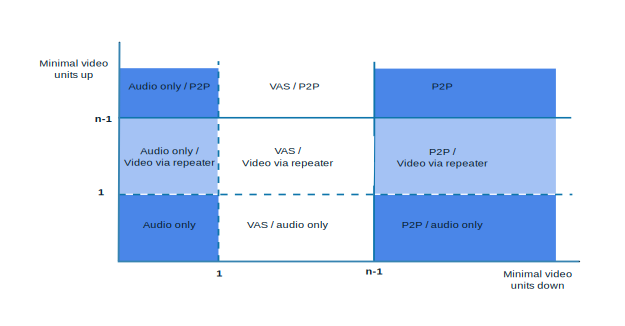
\includegraphics[width=\textwidth]{commcap}
    \caption{The possible services for different upload/download bandwidths. A minimal video is the smallest bitrate where it makes sense to send video. Dark blue is what appear.in can provide today (audio only requires manual configuration), light blue is what's possible with the approach proposed later in this thesis.}
    \label{fig:service-possibilities}
\end{figure}

Continuous presence can be accomplished both in a peer-to-peer topology and centralized topologies, but since a \gls{vas} requires insight into the video streams (or at least, the audio streams) to select who is forwarded at any given time, they are only realizable if all the video streams go through centralized servers. In theory it's possible to expand the system to work over peer-to-peer as well, by having each peer use a low-bandwidth data channel to tell nodes whether it's currently speaking or not, but this requires that video streams can be quickly started, stopped, and that the system gracefully handles collisions without falling over. The problem is non-trivial, as it's essentially a question of distributed consensus. Having a single place that handles the question of who's active is a lot simpler to reason about and implement.

Note that even though video is switched in a \gls{vas}-system, everyone's audio is usually sent to everyone.

\subsection{NAT and Firewalls}

The presence of \gls{nat} makes connection establishment between users harder than necessary, as nodes behind a NAT are not aware of their external IP address and port. The \gls{ice} framework provides two protocols that can be implemented to alleviate parts of the problem; \gls{stun} and \gls{turn}. STUN is a very lightweight protocol used to discover your externally visible network address, while TURN-servers act as intermediaries between users that cannot reach each other directly due to firewalls. TURN servers are often the biggest server expense for WebRTC-based solutions, since the provider have to take the cost for the bandwidth consumed by the users.

For WebRTC, STUN would be needed even in the absence of NATs, since JavaScript does not have any APIs for binding to ports, only for establishing outgoing connections. Thus there's no way for a node to announce the port it's accepting connections to before it has established a connection outward, a chicken-and-egg problem STUN resolves.


\section{The current providers}

A selection of widely known video conversation services with different network architectures is summarized in \autoref{tab:existing-solutions}.

\begin{center}
	\label{tab:existing-solutions}
    \captionof{table}{Network topologies in video conversation services}
	\begin{tabular}{| l | l |}
		\hline
		\textbf{Service} & \textbf{Description} \\ \hline
		appear.in & Browser-based peer-to-peer WebRTC service \\ \hline
		Google Hangouts & Browser-based with Vidyo-powered \gls{sfu} \\ \hline
		Microsoft Skype & Custom application, proprietary peer-to-peer protocol \\ \hline
		Cisco TelePresence & Custom hardware, self-hosted or cloud \glspl{mcu} \\ \hline
	\end{tabular}
\end{center}

Notably absent here is FaceTime, Apple's video conversation service bundled with their devices. FaceTime's absence in this thesis is due to the lack of support for more than two people in a conversation, and the lack of support for non-Apple devices.

We also note that Mozilla just entered the market in collaboration with Telefónica with their Hello service, bundled with recent versions of Firefox\footnote{https://www.mozilla.org/en-US/firefox/hello/}. Hello essentially provides the same service as appear.in, just bundled with the browser. Thus anything we say about appear.in applies to Firefox Hello as well (and all other peer-to-peer WebRTC services), and we'll not consider them separately.

\subsection{appear.in}

appear.in is a free peer-to-peer service built on WebRTC that does not require sign-ups or installation of add-ons to your browser. Due to WebRTC not being fully standardized yet, the service is only available on recent versions of either Google Chrome, Mozilla Firefox or Opera, while the OS-provided browsers (Internet Explorer and Safari) have notably not implemented WebRTC yet.\footnote{Browser support for WebRTC can be tracked at \url{http://iswebrtcreadyyet.com/}} appear.in uses Continuous Presence, while providing the user the option of resizing video streams at will.

appear.in is the only solution studied in this thesis that allow true anonymous communication\footnote{Meaning that the provider doesn't know who you are or who you're talking with.}. The combination of continuous presence and a peer-to-peer topology makes the device and network requirements scale linearly with the number of people in a conversation. The service is limited to maximum 8 people in a conversation.


\subsection{Google Hangouts}

Google Hangouts is alongside appear.in the only other service covered in this thesis based in the browser. Hangouts is a merge of several earlier Google communication solutions like Google Talk, Google+ Messenger and the Hangouts feature from Google+. The service uses a Vidyo-provided \gls{sfu}, and VP8/9 over WebRTC in a non-standard configuration on Chrome \cite{hangouts-webrtc}, and requires a plug-in on other browsers \cite{google-hangouts-support}. A conversation is limited to 10 people. Like was mentioned earlier, Hangouts uses a hybrid-VAS system, where only one party can be shown up big, but the user can override who that is. This strikes a compromise between the high bandwidth requirements of Continuous Presence and the ability to see everyone at the same time.

Hangouts requires you to authenticate with a Google account, which makes anonymous conversations much harder. Hangouts is free to use, but room capacity can be increased to 15 people in the paid Google Apps for Work version.


\subsection{Skype}

Skype is probably the most well-known of the solutions we're looking at, being among the first to offer free video conferencing for personal use way back in 2003. Skype was also among the first to provide a \gls{voip}-service inter-operating with the \gls{pstn}, easing adoption for new users. The Skype topology is peer-to-peer, built on top of the file-sharing protocol powering Kazaa, which was developed by the same founders \cite{skype-history}. The protocol used is proprietary and requires installing the Skype application. For NAT-traversal, Skype initially used other Skype users known as supernodes as intermediaries, performing the same role as TURN-servers in the ICE framework. After the Microsoft acquisition in 2011, Skype dropped the client-hosted supernodes in favor of Microsoft-hosted ones, justified as a means to improve performance and security for users \cite{skype-topo-change}. A Skype conversation has a soft limit on five people for the best user experience, and a hard limit on 10 users.

Skype requires a standalone application to run, which is available on almost all platforms out there, including Windows, Mac, Linux, Android, iOS, Windows Phone, BlackBerry, most tablets, TVs, video game consoles and more. The benefit of native applications is closer access to hardware for more efficient video processing. The downside is often that they -- like Skype -- do not use open protocols, are not standardized and offer no transparency.


\subsection{Cisco}

Cisco offers both on-premises, off-premises and hybrid solutions for video conferencing, aimed at the enterprise market. Video is routed through either self-hosted or cloud \glspl{mcu} or \glspl{sfu}, using \gls{sip} and H.323 for call establishment \cite{cisco-arch}. In the case of only two people in a conversation, calls can be established peer-to-peer. TelePresence enables interoperability with other services that supports SIP and H.323, which through H.320 gateways include devices on legacy networks like the \gls{pstn}, such as ISDN videophones. Their core offering is specialized hardware and dedicated rooms for video conferencing (so-called immersive video conferences), but they also have a free service that can be run on end-user computers using a custom application.


\section{Related Work}

Networking and algorithms related to networking is not a new topic, by any stretch of the imagination, and like in most branches of computer science, it's mostly old problems in a new context.

In this thesis we will borrow heavily from previous work on networking and graph algorithms in general, and flow algorithms in particular. Many algorithmic problems can be solved as a linear program, which as a problem was first solved by Fourier in 1827 \cite{sierksma2001linear}. Another solution, the simplex algorithm, was first introduced by G.B. Dantzig in 1947 \cite{sierksma2001linear}, and serves as the basis for the \gls{lp}-solver we'll use for in the sample implementation. Multi-commodity flow networks was introduced to me in \cite{ahuja1988network} by Ahuja, Magnanti and Orlin, which establishes the fundamentals for the approach proposed later in this thesis. The simplex algorithm has been widely adopted for its ease of implementation on computers, and years of exponential growth of computer performance has made solving increasingly large problem sets feasible.

A study at Chalmers in 2014 \cite{tree-topology-webrtc} investigated the feasibility of utilizing normal nodes in a video conference as supernodes, routing traffic from less powerful nodes through these nodes to reduce network load. The authors concluded that such a solution is feasible given proper supernode selection, which gives even greater possibilities for a solution utilizing dynamic topologies like presented in this thesis. Pushing as much traffic as possible over client-provided supernodes lowers the cost for the provider, and enables better quality for the users since peers can be closer to each other than to the closest data center. As the study concluded with supernodes being feasible and beneficial, the approach outlined here is developed to be flexible enough to allow nodes to forward video to other nodes.
